\documentclass{standalone}
\usepackage{picture,color}
\usepackage{graphicx}
\graphicspath{{./initialization/}}
\setlength{\unitlength}{1in}
\renewcommand{\rmdefault}{phv} % Arial
\renewcommand{\sfdefault}{phv} % Arial


\begin{document}
\begin{picture}(6.3, 5.2)(0,-5.4)

\put(0.2, -0.9){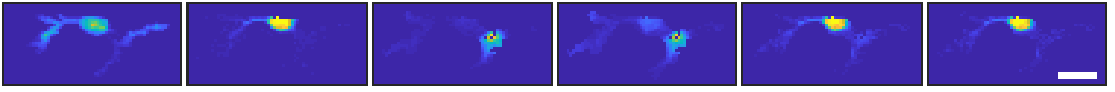
\includegraphics[height=0.504in]{results_ai_3.pdf}}
\put(0.015, -0.43){\large\textbf{A}}
\put(0.35, -0.35){EM footprint}
\put(1.36, -0.35){ground truth}
\put(2.26, -0.35){semi-NMF,RSS}
\put(3.25, -0.35){semi-NMF,wRSS}
\put(4.45, -0.35){EASE,RSS}
\put(5.4, -0.35){EASE,wRSS}
\put(0.8, -0.63){\color{red}\vector(1,0){0.01}}
\put(1.8, -0.63){\color{red}\vector(1,0){0.01}}
\put(2.8, -0.63){\color{red}\vector(1,0){0.01}}
\put(3.8, -0.63){\color{red}\vector(1,0){0.01}}
\put(4.8, -0.63){\color{red}\vector(1,0){0.01}}
\put(5.9, -0.63){\color{red}\vector(1,0){0.01}}


% \put(1.3, -0.25){Relative size of EM components}

\put(0.185, -3){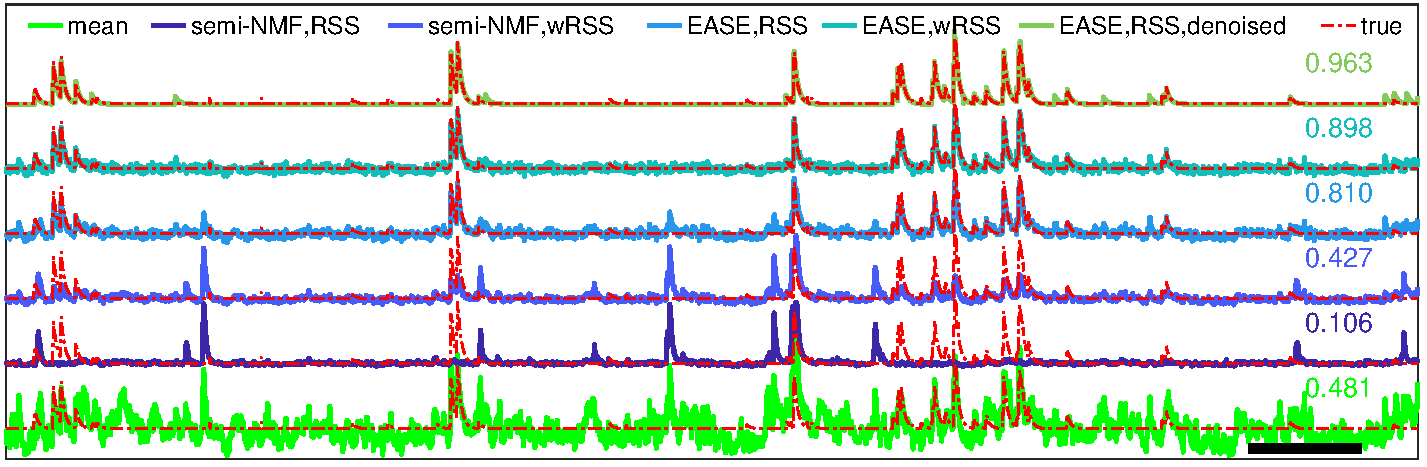
\includegraphics[height=2in]{results_ci_3.pdf}}
\put(0.015, -1.05){\large\textbf{B}}
\put(0.35, -2.98){\color{red}\vector(0,1){0.01}}
\put(1., -2.98){\color{red}\vector(0,1){0.01}}
\put(1.08, -2.98){\color{red}\vector(0,1){0.01}}
\put(2.28, -2.98){\color{red}\vector(0,1){0.01}}
\put(2.73, -2.98){\color{red}\vector(0,1){0.01}}
\put(3.1, -2.98){\color{red}\vector(0,1){0.01}}
\put(3.5, -2.98){\color{red}\vector(0,1){0.01}}
\put(4.08, -2.98){\color{red}\vector(0,1){0.01}}
\put(4.0, -2.98){\color{red}\vector(0,1){0.01}}
\put(5.8, -2.98){\color{red}\vector(0,1){0.01}}
\put(6.2, -2.98){\color{red}\vector(0,1){0.01}}


\put(0.05, -5.4){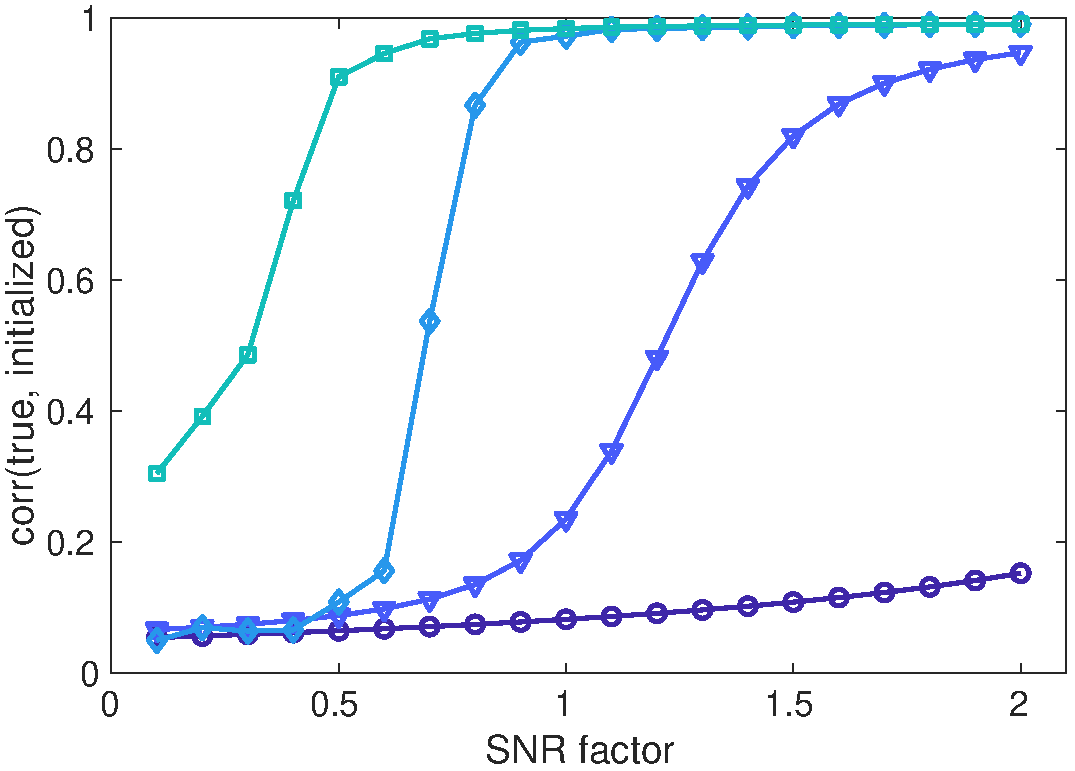
\includegraphics[height=2.22in]{ai_corr_3.pdf}}
\put(1.15, -3.15){Spatial component}
\put(3.32, -5.4){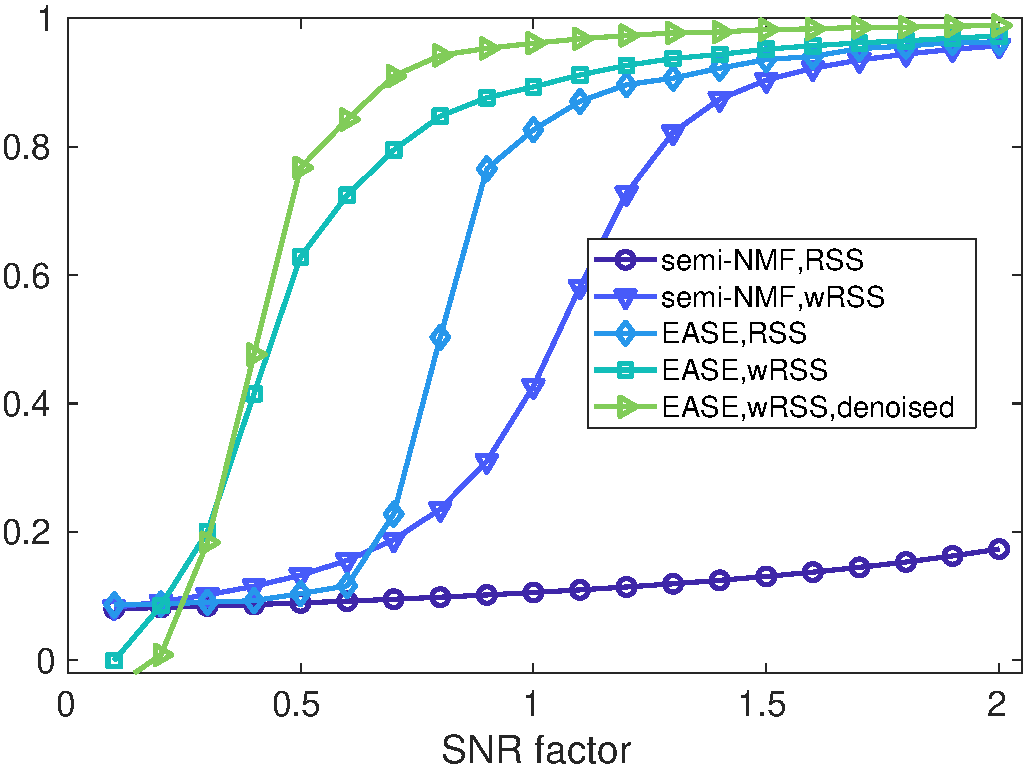
\includegraphics[height=2.22in]{ci_corr_3.pdf}}
\put(0.015, -3.2){\large\textbf{C}}
\put(3.2, -3.2){\large\textbf{D}}
\put(4.2, -3.15){Temporal component}
% % slice number 
% \put(0.9, -2.3){{slice 1}}
% \put(2.3, -2.3){{slice 2}}
% \put(3.7, -2.3){{slice 3}}
% \put(0.01, -2.3){\large\textbf{B}}

% % neuron 1
% \put(0.35, -2.92){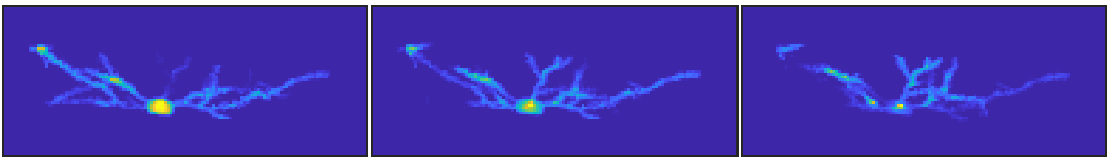
\includegraphics[width=4.2in]{example_1.pdf}}
% \put(0.2, -2.64){\rotatebox{90}{\color{red}8}}

% % neuron 2 
% \put(0.35, -3.53){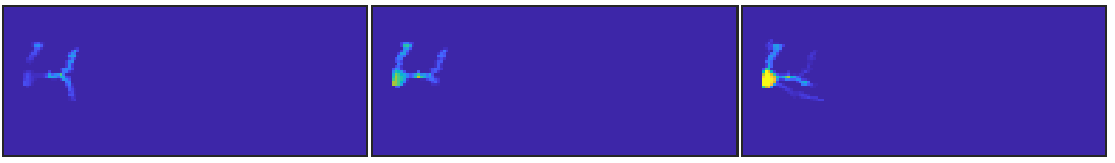
\includegraphics[width=4.2in]{example_2.pdf}}
% \put(0.2, -3.31){\rotatebox{90}{\color{green}200}}

% % neuron 3 
% \put(0.35, -4.14){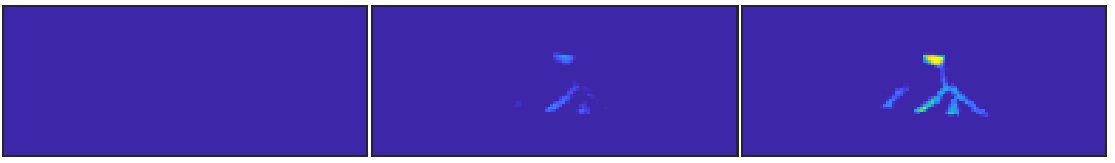
\includegraphics[width=4.2in]{example_3.pdf}}
% \put(0.2, -3.92){\rotatebox{90}{\color{cyan}409}}

% % neuron 4
% \put(0.35, -4.75){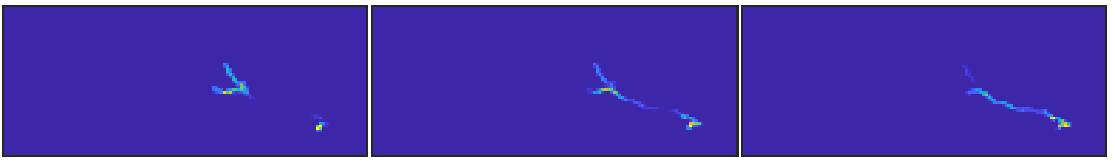
\includegraphics[width=4.2in]{example_4.pdf}}
% \put(0.2, -4.57){\rotatebox{90}{\color{magenta}1033}}

% % neuron 5
% \put(0.35, -5.36){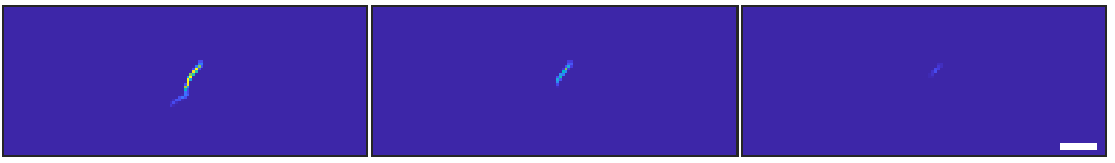
\includegraphics[width=4.2in]{example_5.pdf}}
% \put(0.2, -5.23){\rotatebox{90}{\color{blue}30000}}
\end{picture}
\end{document}\grid
